\documentclass{beamer}
\usetheme{Madrid}

\usepackage{tikz}

\title[Physics Problem Solving]{Physics Problem Solving}
\author{Eason Shao \and Lev Shabalin}
\institute[]{Physics Problem Solving Society\\St Paul's School}
\date{22.04.2024}

\AtBeginSection[]
{
    \begin{frame}
        \frametitle{Table of Contents}
        \tableofcontents[currentsection]
    \end{frame}
}

\begin{document}

    \frame{\titlepage}
    
    \begin{frame}
        \frametitle{Table of Contents}
        \tableofcontents
    \end{frame}
    
    \section{Fluid Pressure}
        \begin{frame}
            \frametitle{About Fluid Pressure}
            We have previously discussed (in our first session) that the static pressure that fluid exerts only depends on gravitational acceleration $g$, fluid density $\rho$, and the depth $h$ (to the free surface).\pause
        
            \begin{alertblock}{Formula for Fluid Pressure}
                The pressure exerted by a certain liquid with density $\rho$ at depth $h$ is given by the following formula:
                $$p = \rho g h.$$
            \end{alertblock}\pause
        
            \begin{block}{Remark}
                Static fluid pressure does not depend on the shape of the container, the total mass, or the surface area of the liquid.
            \end{block}
        \end{frame}
        
        \begin{frame}
        \frametitle{About Fluid Pressure}
            However, it is not intuitive why the pressure exerted by the liquid at the bottom of the liquid, times by the area (which is the force exerted by the liquid), is different from the weight of the liquid:
            $$
            F = pA = \rho h A g \neq W = mg = \rho V g
            $$
            for containers which does not satisfy $V = Ah$.
        \end{frame}
        
        \begin{frame}
            \frametitle{About Fluid Pressure}
            Thanks to a conversation with Mr Swartzentruber, we have came up with a somewhat-nice explanation of why.\pause
        
            \begin{figure}
                \centering
                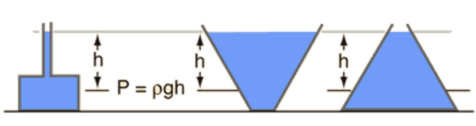
\includegraphics[width=0.5\textwidth]{FluidPressure.png}
                \caption{Some Containers}
                \label{fig:FluidContainer}
            \end{figure}\pause
                
            \begin{exampleblock}{First Container}\pause
                \begin{itemize}
                    \item The liquid would have exerted pressure on the top flat surface, and hence by N3 will receive a reaction from the container, downwards.\pause
                    \item To let the resultant force be equal to zero, not only does the container has to provide an upward force equal to the weight at the bottom, but also some extra to compensate for the downwards force.
                \end{itemize}
            \end{exampleblock}
        \end{frame}

        \begin{frame}
            \frametitle{About Fluid Pressure}
            Similar explanations can be given for the other two containers, where the side walls either give support reactions for the weight, or give reactions downwards which requires more force exerted at the bottom.\pause
            
            \begin{alertblock}{Pressure in a Non-Column Container}
                Fluid exerts static pressure in a non-column container, as if a column of liquid with the same depth is on the top of the bottom of the container.
            \end{alertblock}
        \end{frame}
    
    \section{Eason's Question}
        \begin{frame}
            \frametitle{Eason's Question}
            
            There is a step of height $h$, with a smooth pulley attached on top. A block of mass $M$ rests on a smooth ground, with distance $x$ from the step. There is a light string connecting the mass to the pulley, and there is a constant force $F$ applied to the string (which is passed on to the mass by the tension).\pause
            
            Find the work done by the tension in the string as it pulls the mass to just below the step, assuming that the mass does not lift off from the ground (i.e. $F \leq Mg$).\pause

            \begin{figure}
                \centering
                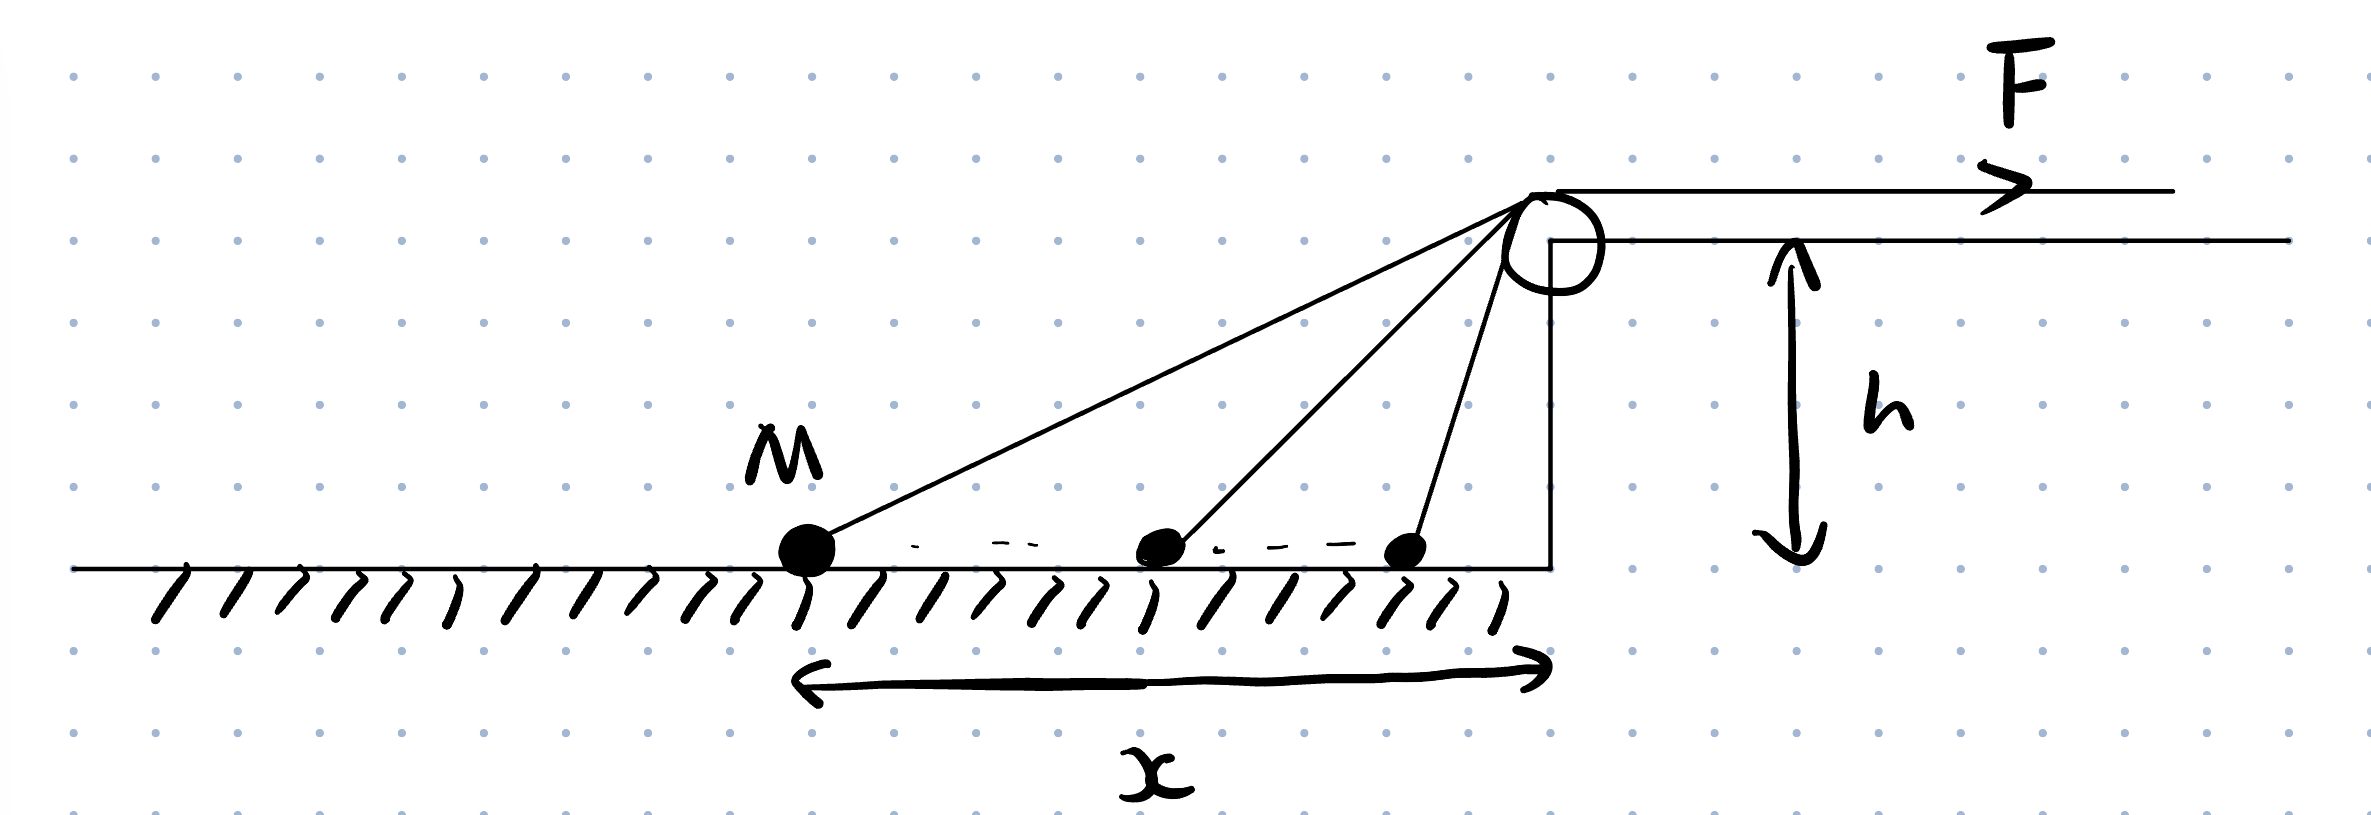
\includegraphics[width=0.75\textwidth]{Diagram.jpg}
                \caption{Diagram for Question}
                \label{fig:MyQ}
            \end{figure}
        \end{frame}

        \begin{frame}
            \frametitle{Solutions}

            As Eason mentioned in Google Classroom, in fact there are two very different solutions to this question.\pause

            The most straightforward solution uses the following integration formula:\pause
            \begin{alertblock}{Work Done}
                Work done $W$ by a force $\mathbf{F}$ over displacement $\mathbf{x}$ is defined by
                $$
                W = \int \mathbf{F} \cdot \mathrm{d} \mathbf{x} = \int F \cos \theta \mathrm{d} x.
                $$
            \end{alertblock}
        \end{frame}

        \begin{frame}
            \frametitle{Solutions}
            
            If we set $l$ as the distance of mass $M$ from the step, and $\theta$ as the angle between the string and the horizontal ground, we will have
            $$
            \theta = \arctan{\frac{h}{l}}.
            $$\pause

            Therefore,
            $$
            \cos \theta = \frac{l}{\sqrt{h^2+l^2}}.
            $$\pause

            Therefore, we will have
            \begin{align*}
                W &= \int F \cos \theta \mathrm{d}x \\
                  \onslide<4->{&= F \int_{0}^{x} \cos \theta \mathrm{d}l} \\
                  \onslide<5->{&= F \int_{0}^{x} \frac{l}{\sqrt{h^2 + l^2}} \mathrm{d}l.}
            \end{align*}
        \end{frame}
        
        \begin{frame}
            \frametitle{Solutions}

            We may notice that
            $$
            l = \frac{1}{2} \frac{\mathrm{d}}{\mathrm{d}l} (h^2 + l^2).
            $$\pause

            Therefore, 
            \begin{align*}
                W &= F \int_{0}^{x} \frac{l}{\sqrt{h^2 + l^2}} \mathrm{d}l\\
                  \onslide<3->{&= \frac{1}{2} F \int_{h^2}^{x^2+h^2} \frac{\mathrm{d}(h^2+l^2)}{\sqrt{h^2 + l^2}}}\\
                  \onslide<4->{&= \frac{1}{2} F \int_{h^2}^{x^2+h^2} \frac{\mathrm{d}u}{\sqrt{u}}}\\
                  \onslide<5->{&= F \left[\sqrt{u}\right]_{h^2}^{x^2 + h^2}}\\
                  \onslide<6->{&= F \left(\sqrt{x^2 + h^2} - h\right)}.
            \end{align*}
        \end{frame}

        \begin{frame}
            \frametitle{Why this result?}

            $$
            W = F \left(\sqrt{x^2 + h^2} - h\right)
            $$
            \pause
            
            The term $\sqrt{x^2 + h^2}$ is the original distance of the mass from the pulley, while the term $h$ is the final distance of the mass from the pulley.\pause

            The difference is the distance that the rope has shortened.\pause

            Imagine if I were pulling the rope on a free end on the right. Then this distance will be the distance I have moved.\pause

            Energy is conserved. The work I done to the rope, will all be transferred to the work done by the tension to the mass.\pause

            I pulled with force $F$ over the distance of $\sqrt{x^2 + h^2} - h$.\pause

            Work done is $W = F \left(\sqrt{x^2 + h^2} - h\right)$.
        \end{frame}
        
    \section{Easter Question Pack (If we have time) }
        \begin{frame}
            \frametitle{Q1 (2016 R1 q)}

            \begin{block}{Question 1.}
                A particle, mass $m$, slides down the smooth track, from a height $H$ under gravity. It is to complete a circular trajectory of radius $R$ when reaching its lowest point. Determine the smallest value of $H$.\pause
    
                \begin{figure}[!h]
                    \begin{center}
                        \begin{tikzpicture}[scale=1.5]
                            \draw[dashed] (-3.5,0) -- (-0.3,0);
                            \draw[domain=-3:-0.2] plot (\x, {-0.1*\x*\x*\x});
                            \draw (-0.3,1) circle (1cm);
                            \draw[->] (-0.3,0) -- (1.5,0);
                            \draw (1.5,0) -- (2,0);
                            \draw [->] (0.7,1) -- (0.7,1.01);
                            \draw [->] (-1.3,1.01) -- (-1.3,1);
                            \draw [<->] (-3.2, 0) -- (-3.2,2.7);
                            \draw[fill=black] (-2.7,2.2) circle (0.08cm);
                            \node at (-3.5,1.35) {$H$};
                            \node at (-2.4,2.2) {$m$};
                            \draw[->] (-2.5,1.563) -- (-2.498,1.56);
                            \draw [<->] (-0.3,1) -- (0.407,1.707);
                            \node at (0.1,1.6) {$R$};
                            %\node at (-0.9,-1) {\textbf{Figure 1(q)}};
                        \end{tikzpicture}
                    \end{center}
                    \caption{2016 R1 q}
                    \label{fig:16fq}
                \end{figure}
            \end{block}
        \end{frame}

        \begin{frame}
            \frametitle{Q1 (2016 R1 q)}
            \begin{exampleblock}{Solution}
                If the mass is to complete the circular path, then at the top of the circle we require the normal contact force from the constraining circle to satisfy $N\geq 0$.\pause
            
                The centripetal force must be equal to the forces acting on the mass in order for its path to be circular, so
                $$\frac{mv^2}{R} = N + mg.$$\pause
                
                The smallest value for $v$ while still satisfying $N\geq0$ occurs when $N=0$. Therefore,
                \begin{align*}
                    \frac{mv^2}{R}&\geq mg,\\
                    \onslide<4->{v^2 &= Rg.}
                \end{align*}
            \end{exampleblock}
        \end{frame}

        \begin{frame}
            \frametitle{Q1 (2016 R1 q)}

            \begin{exampleblock}{Solution}
                By the conservation of energy, the gravitational potential energy lost by the particle from the top of the track to the top of the circle is equal to the kinetic energy gained.
                $$mg(H-2R) = \frac{1}{2}mv^2.$$\pause
                
                Substituting the expression we have for $v^2$ from above, 
                \begin{align*}
                    mg(H-2R) &= \frac{1}{2}mRg,\\
                    \onslide<3->{H-2R &= \frac{1}{2}R,}\\
                    \onslide<4->{H &= \frac{5}{2}R.}
                \end{align*}
            \end{exampleblock}
        \end{frame}
\end{document}